\documentclass[11pt]{article}
%\usepackage{fullpage,url}
\usepackage{url}
\usepackage{amsmath}
\usepackage{graphicx}
\usepackage{caption}
\usepackage{subcaption}

\usepackage[letterpaper,top=1in,bottom=1in,left=1in,right=1in,nohead]{geometry}

\setlength{\parindent}{0in}
\setlength{\parskip}{6pt}
\bibliographystyle{plain}

\DeclareMathOperator{\E}{E}
\DeclareMathOperator{\Var}{Var}
\DeclareMathOperator{\Unif}{Unif}
\DeclareMathOperator{\shrink}{shrink}

\begin{document}
\thispagestyle{empty}
{\large{\bf CS7640: Advanced Image Processing \hfill Danny Perry}}\\

{\LARGE{\bf Sparse coding and non-local image denoising}}
\vspace{0.2\baselineskip}
\hrule

\section{Introduction}
One of the classic problems in image analysis is image denoising.
Some of the landmark approaches to image denoising include \cite{perona1990scale} and \cite{rudin1992nonlinear}.
Each of these model the denoising problem using partial differential equations, as anisotropic diffusion in the first and total variation over the image in the second. 

Another approach to image denoising is to "learn" what a certain patch distribution looks like, and then to take the expectation of that distribution.
\cite{buades2005non} introduce the algorithm NL-means that makes use of this kind of learning approach.
It is defined by this formula:

\begin{equation}
NL[u](x) = \frac{1}{C(x)} \int_{\Omega} \exp( (-G_a*|u(x+.)-u(y+.)|^2)(0) / h^2 ) u(y) dy
\end{equation}

where $u(\cdot)$ is the noisy image, $x,y,z\in \Omega$, $G_a$ is a Gaussian kernel and $h$ is a filtering parameter, and 
\begin{equation*}
C(x) = \int_{\Omega} \exp( (-G_a*|u(x+.)-u(z+.)|^2)(0) / h^2 ) dz,
\end{equation*}

For a discrete noisy image $v = {v(i) | i \in I}$,
\begin{equation}
NL[v](i) = \sum_{j \in I} w(i,j) v(j),
\end{equation}
where
\begin{equation*}
w(i,j) = \frac{1}{Z(i)} \exp( -||v(N_i)-v(N_j)||_2^2 / h^2 ),
\end{equation*}
and
\begin{equation*}
Z(i) = \sum_k \exp( -||v(N_i)-v(N_k)||_2^2 / h^2 )
\end{equation*}

A closely related approach was presented in \cite{awate2006unsupervised}, where instead of finding the expectation of the patch distribution, the entropy of the patch was minimized using gradient descent.

Denoising using sparse representation of images can be described in a similar way.
Instead of modeling the original distribution of the (potentially noisy) patches, sparse representation restricts the distribution of the patch to a subspace defined by an overcomplete dictionary.  
A smoothing over this restricted representation is then performed.
K-SVD \cite{aharon2005k} is one popular approach to approximating the sparse representation, which has been shown to have a noise rejection capability \cite{elad2006image}. 
Such a denoising approach is presented in \cite{elad2006image}.

I've implemented the NL-means and K-SVD-based denoising algorithms using the Julia language \cite{julia2012}, a language similar in syntax to Matlab, but with some potential speed advantages.
Here I evaluate both algorithms by denoising a variety of images.

\section{Results}

Each algorithm was run against several images.  
The results of three of those images are show below: the cameara man image (Figure \ref{fig:cameraman:dn}), a sailboat image (Figure \ref{fig:sailboat:dn}), and a slice of a seismic image (Figure \ref{fig:slice:dn}).

For the cameraman and sailboat images Gaussian noise with $\sigma^2=100$ was added to the image.
This was done to make the denoising effect more apparent.

For the slice of seismic volume, the image was equalized to bring out the horizons.
Denoising was applied with the goal of making the horizons appear more continuous.
The seismic image is a slice taken from the Netherlands data set found on the OpendTect data repository \cite{opendTectWeb}.

\begin{figure}
\centering
\graphicspath{{images/}}
\begin{subfigure}[b]{0.4\textwidth}
\centering
\includegraphics[width=\textwidth]{sailboat_256}
\caption{Original}
\label{sail:original}
\end{subfigure}
\begin{subfigure}[b]{0.4\textwidth}
\centering
\includegraphics[width=\textwidth]{sailboat_256_10}
\caption{Noisy}
\label{sail:noise}
\end{subfigure}
\begin{subfigure}[b]{0.4\textwidth}
\centering
\includegraphics[width=\textwidth]{sailboat_10_nl}
\caption{NL-Means}
\label{sail:nl}
\end{subfigure}
\begin{subfigure}[b]{0.4\textwidth}
\centering
\includegraphics[width=\textwidth]{sailboat_256_10_ksvd}
\caption{K-SVD-based Denoising}
\label{sail:ksvd}
\end{subfigure}
\caption{Results of each algorithm on a noisy image of a sailboat.}
\label{fig:sailboat:dn}
\end{figure}


\subsection{NL-Means algorithm}

The NL-means algorithm is very straightforward to implement.
However, the algorithm is deceivingly costly.  
As summarized above, the naive implementation requires $O(n^4)$, with an image of size $n$ by $n$.

Luckily, for a large class of images, the pixels most similar to a specific pixel neighborhood will be those in the immediate vicinity.
This property is known as the "mixing property" in a markov random field \cite{wikiMRF}.

For this reason, as noted in \cite{buades2005non}, when running the algorithm a search window is usually specified much smaller than the entire image. 
\cite{buades2005non} specifically recommends a search window of size $21$ by $21$, and a patch size of $7$ by $7$.
I did some experimentation but essentially use these or similar parameters.

Besides the patch size and search window size, the NL-means algorithm requires an additional two parameters: $\sigma^2$, the variance of the Gaussian kernel, and $h$ the support of the similarity window.
I experimented with various values for these parameters as well, and show some results.

Results on various images are shown, for example, the result of using NL-Means on the sailboat image is shown in Figure \ref{sail:nl}.
Results for the cameraman image is shown in Figure \ref{camera:nl}, and for the slice of seismic imagery is shown in Figure \ref{slice:nl}.
Note how the algorithm is able to smooth while still retaining details in the image.

The least sensitive parameter is probably the Gaussian kernel variance, $\sigma^2$.
Adjusting that parameter by small amounts seemed to influence the outcome in smaller steps than $h$.
For example, Figure \ref{fig:boat:varsigma} shows some results of varying the kernel variance.
What is essentially happening here is that the similarity between two patches is being slightly modified with the different kernels. 
With a Gaussian kernel with low variance, differences will be emphasized, providing less opportunity for blurring.
With a Guassian kernel with high variance, the differences will be less strong, providing more opportunity for blurring.

\begin{figure}
\centering
\graphicspath{{images/}}
\begin{subfigure}[b]{0.4\textwidth}
\centering
\includegraphics[width=\textwidth]{boatnoisy_2_10_0p1_0p2}
\caption{$\sigma^2=0.2$}
\end{subfigure}
\begin{subfigure}[b]{0.4\textwidth}
\centering
\includegraphics[width=\textwidth]{boatnoisy_2_10_0p1_0p6}
\caption{$\sigma^2=0.6$}
\end{subfigure}
\begin{subfigure}[b]{0.4\textwidth}
\centering
\includegraphics[width=\textwidth]{boatnoisy_2_10_0p1_1p0}
\caption{$\sigma^2=1.0$}
\end{subfigure}
\begin{subfigure}[b]{0.4\textwidth}
\centering
\includegraphics[width=\textwidth]{boatnoisy_2_10_0p1_1p4}
\caption{$\sigma^2=1.4$}
\end{subfigure}
\caption{Varying the $\sigma^2$ parameter for the NL-Means algorithm, with $h=0.1$ constant.}
\label{fig:boat:varsigma}
\end{figure}

The filter support parameter $h$ is much more sensitive to a given value.
Smaller changes in $h$ evoke large changes in the sharpness/bluriness of the image.
For example \ref{fig:boat:varh} shows some results with varying support sizes.
Similarly to $\sigma^2$, as the value increases there is more smoothing going on in the images, but the effect appears to be much more sensitive to the changes in input.

\begin{figure}
\centering
\graphicspath{{images/}}
\begin{subfigure}[b]{0.4\textwidth}
\centering
\includegraphics[width=\textwidth]{boatnoisy_2_10_0p2_0p2}
\caption{$h=0.2$}
\end{subfigure}
\begin{subfigure}[b]{0.4\textwidth}
\centering
\includegraphics[width=\textwidth]{boatnoisy_2_10_0p6_0p2}
\caption{$h=0.6$}
\end{subfigure}
\begin{subfigure}[b]{0.4\textwidth}
\centering
\includegraphics[width=\textwidth]{boatnoisy_2_10_1p0_0p2}
\caption{$h=1.0$}
\end{subfigure}
\begin{subfigure}[b]{0.4\textwidth}
\centering
\includegraphics[width=\textwidth]{boatnoisy_2_10_1p4_0p2}
\caption{$h=1.4$}
\end{subfigure}
\caption{Varying the $h$ parameter for the NL-Means algorithm, with $\sigma^2=0.2$ constant.}
\label{fig:boat:varh}
\end{figure}


\subsection{K-SVD Based Denoising}

The K-SVD denoising algorithm is a little more complex than the NL-Means.
While the algorithm coding isn't horrible, the interaction of the various parts make it a little more sensitive to various parameters, etc.

Also, similar to NL-Means, theoretically you can get some pretty bad upper bounds on runtime and storage requirements.
A naive impelementation that does not make use of a sparse matrix data structure will quickly use a surprising amount of memory, if a large dictionary and a large number of image patches are used (requiring the sparse representation vector for all patches to be a large matrix in both dimensions).

However, \cite{elad2006image} recommends some specific parameters that help to minimize those costs.
For example, they use smaller $256$ by $256$ size images to limit the number of patches to encode.
For larger $512$ by $512$ images they recommend skipping every other line, again to keep that dimension to a reasonable figure.
Other recommended parameters include using an overcomplete dictionary with $256$ atoms.
Again, this size keeps the space and runtime requirements reasonable.
Other parameters that need tuning include the sparsity limit (they recommend using under $6$), the limit placed on the residual after each matching pursuit and K-SVD iteration (recommended to be adjusting according to the variance of the noise model $\sigma^2$, for example $(1.15*\sigma)^2$), as well as the relaxation coefficient (they recommend this being a ratio of the noise model - for example $30/\sigma$).
I use these or similar parameters for the results shown here.

Results are shown for the K-SVD-based denoising in Figures \ref{sail:ksvd},\ref{camera:ksvd}, and \ref{slice:ksvd}.
You will note that the K-SVD denoised images are very blurry.
While I was able to successfully decompose and reconstruct an image using the a dictionary and the K-SVD algorithm, I had some trouble tuning the parameters for denoising the images, and because the assignment is due, I unfortunately present these results as is.

I was able to implement the denoising using a random dictionary, a DCT based dictionary, and a dictionary constructed from the noisy images itself.
Here I show some results comparing using the DCT and noisy-image based dictionaries.
Figure \ref{fig:cameraman:sparse} compares the denoising results using the different dictionaries on the noisy cameraman image.
Likewise, Figure \ref{fig:sailboat:sparse} compares some results using the different dictionaries on the noisy sailboat image.



\begin{figure}
\centering
\graphicspath{{images/}}
\begin{subfigure}[b]{0.4\textwidth}
\centering
\includegraphics[width=\textwidth]{cameranoisy_3_8_dct}
\caption{Denoising usine DCT-based dictionary.}
\label{camera:sparse:dct}
\end{subfigure}
\begin{subfigure}[b]{0.4\textwidth}
\centering
\includegraphics[width=\textwidth]{cameranoisy_3_8_ksvd}
\caption{Noisy-image based dictionary (K-SVD).}
\label{camera:sparse:ksvd}
\end{subfigure}
\caption{Results of using the sparse dictionary based denoising algorithm on the cameraman image.  One used a DCT-based dictionary while the other used a dictionary trained using K-SVD on the noisy image.  The differences are subtle, and difficult to convey visually.}
\label{fig:cameraman:sparse}
\end{figure}


\begin{figure}
\centering
\graphicspath{{images/}}
\begin{subfigure}[b]{0.4\textwidth}
\centering
\includegraphics[width=\textwidth]{cameraman_256}
\caption{Original}
\label{camera:original}
\end{subfigure}
\begin{subfigure}[b]{0.4\textwidth}
\centering
\includegraphics[width=\textwidth]{cameraman_256_10}
\caption{Noisy}
\label{camera:noise}
\end{subfigure}
\begin{subfigure}[b]{0.4\textwidth}
\centering
\includegraphics[width=\textwidth]{cameraman_10_nl}
\caption{NL-Means}
\label{camera:nl}
\end{subfigure}
\begin{subfigure}[b]{0.4\textwidth}
\centering
\includegraphics[width=\textwidth]{cameraman_256_10_ksvd}
\caption{KSVD-based denoising}
\label{camera:ksvd}
\end{subfigure}
\caption{Results of each algorithm on a noisy image of a cameraman.}
\label{fig:cameraman:dn}
\end{figure}

\begin{figure}
\centering
\graphicspath{{images/}}
\begin{subfigure}[b]{0.4\textwidth}
\centering
\includegraphics[width=\textwidth]{boatnoisy_3_8_dct}
\caption{Denoising usine DCT-based dictionary.}
\label{boat:sparse:dct}
\end{subfigure}
\begin{subfigure}[b]{0.4\textwidth}
\centering
\includegraphics[width=\textwidth]{boatnoisy_3_8_ksvd}
\caption{Noisy-image based dictionary (K-SVD).}
\label{boat:sparse:ksvd}
\end{subfigure}
\caption{Results of using the sparse dictionary based denoising algorithm on the sailboat image. As in Figure \ref{fig:cameraman:sparse}, the differences are subtle, and difficult to see visually.}
\label{fig:sailboat:sparse}
\end{figure}



\begin{figure}
\centering
\graphicspath{{images/}}
\begin{subfigure}[b]{0.5\textwidth}
\centering
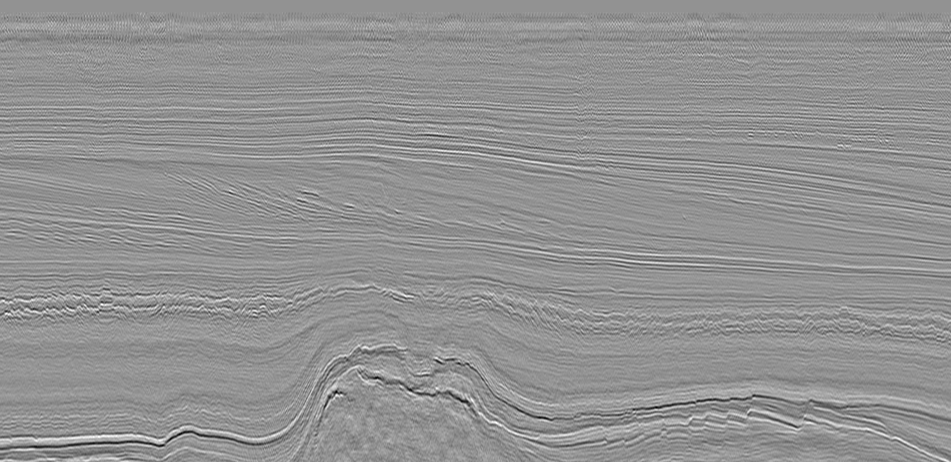
\includegraphics[width=\textwidth]{slice}
\caption{Original}
\label{slice:original}
\end{subfigure}
\begin{subfigure}[b]{0.5\textwidth}
\centering
\includegraphics[width=\textwidth]{slice_eq_256}
\caption{Equalized no denoising}
\label{slice:noise}
\end{subfigure}
\begin{subfigure}[b]{0.5\textwidth}
\centering
\includegraphics[width=\textwidth]{slice_eq_nl}
\caption{NL-Means}
\label{slice:nl}
\end{subfigure}
\begin{subfigure}[b]{0.5\textwidth}
\centering
\includegraphics[width=\textwidth]{slice_eq_256_ksvd}
\caption{K-SVD-based denoising}
\label{slice:ksvd}
\end{subfigure}
\caption{Results of each algorithm on a slice of a seismic volume from the OpendTect project \cite{opendTectWeb}. The slice has been equalized prior to smoothing to enhance appearance of horizons.}
\label{fig:slice:dn}
\end{figure}


\section{Conclusion}

The classic problem of denoising has been attacked from a variety of approaches.
Here we've presented two additional methods of denoising - NL-Means based on the expectation of the distribution of a patch in the image, and Sparse dictionary based denoising - using the decomposition of the image using an overcomplete dictionary to denoise.
While the results here for the overcomplete dictionary aren't overwhelmining satsifying, the exercise did convey the flavor of the approach.
And by considering the original results, and the results presented here for NL-Means, one can conclude that both techniques provide for interesting approaches to a classic problem.


\bibliography{sparse}

\end{document}
